\documentclass[11pt]{article}
\usepackage[fleqn]{amsmath}\textwidth 6.5in
\oddsidemargin -0.25in
%\evensidemargin -0.5in
\topmargin -0.25in
\textheight 9.0in

\newcommand{\docname}{\bf wvs-048r5}
\newcommand{\docdate}{27 April 2009}

\usepackage{graphicx}

\usepackage{floatflt}

\begin{document}

%\tracingcommands=1
\newlength{\hW} % heading box width
\newlength{\pW} % page number field width
\settowidth{\hW}{\docname}
\settowidth{\pW}{Page \pageref{lastpage}\ of \pageref{lastpage}}
\ifdim \pW > \hW \setlength{\hW}{\pW} \fi
\makeatletter
\def\@biblabel#1{#1.}
\newcommand{\ps@twolines}{%
  \renewcommand{\@oddhead}{%
    \docdate\hfill\parbox[t]{\hW}{{\hfill\docname}\newline
                          Page \thepage\ of \pageref{lastpage}}}%
\renewcommand{\@evenhead}{}%
\renewcommand{\@oddfoot}{}%
\renewcommand{\@evenfoot}{}%
}%
\makeatother
\pagestyle{twolines}

\vspace{-10pt}
\begin{tabbing}
\phantom{References: }\= \\
To: \>Bill\\
Subject: \>Different solution for $\phi$--$H$ calculation in {\tt metrics\_m}\\
From: \>Van Snyder\\
\end{tabbing}

\parindent 0pt \parskip 10pt
\vspace{-20pt}

\begin{floatingfigure}{3.75in}
{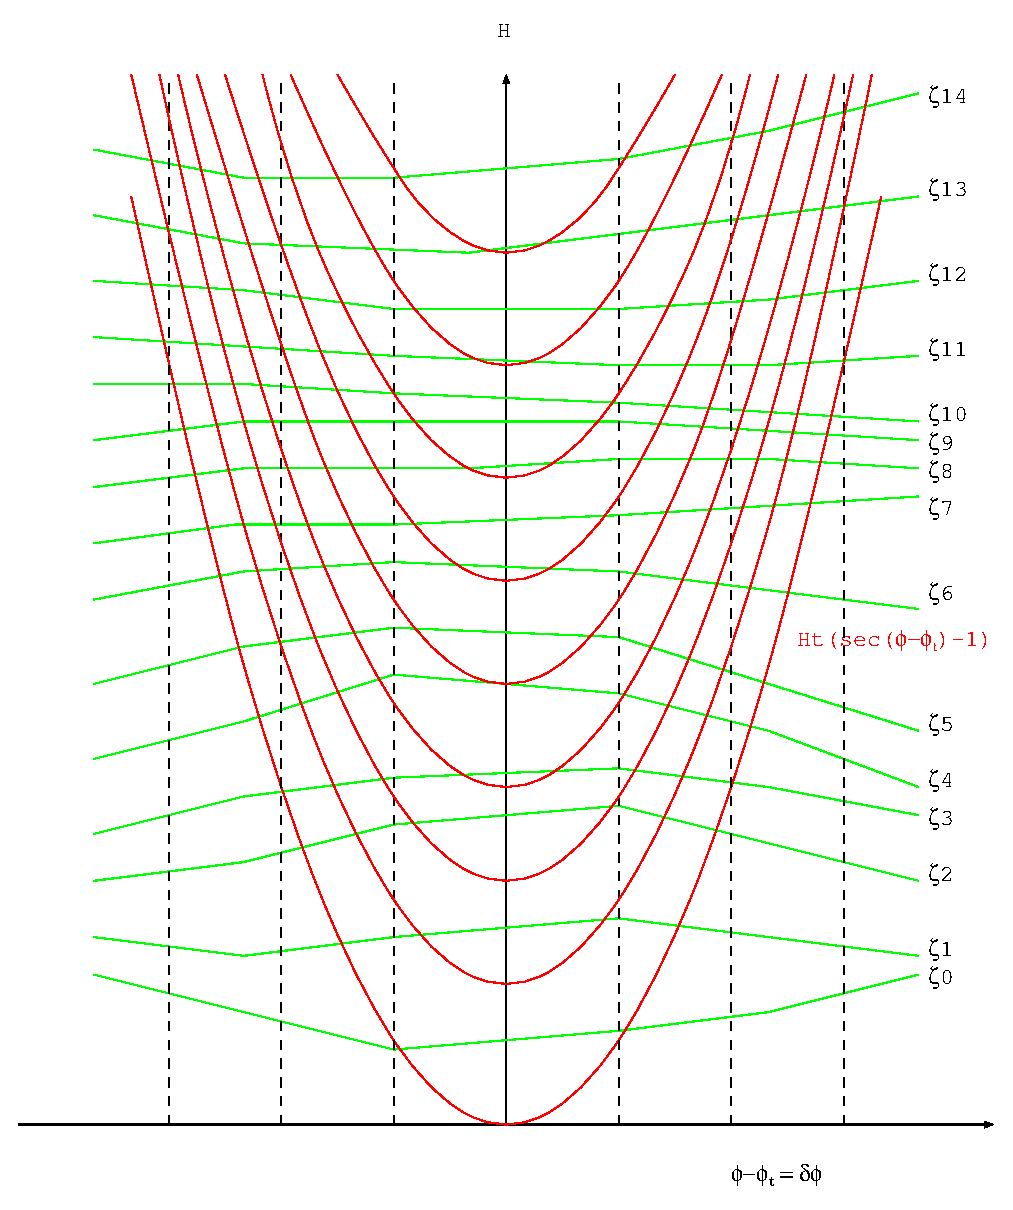
\includegraphics[width=3.5in,height=4.5in,clip]{./wvs-048-grid2.eps}}
\end{floatingfigure}

We want to solve for $\phi$ and $H$ at the intersections of the line of
sight with constant-$\zeta$ surfaces.

I drew the picture of the line of sight intersecting the $\zeta$ surfaces
in cartesian $\phi$--$H$ co\"{o}rdinates instead of polar 
$\phi$--$\zeta$ co\"{o}rdinates.  In this diagram, the con\-stant-$\zeta$
surfaces are the green lines, the line of sight is the red line, and the
temperature $\phi$ basis $\phi_1 \dots \phi_n$ is the vertical black
lines.  Therefore the values of $H$ in the {\tt H\_ref} array appear at
the intersections of the green lines and the vertical black lines.

Assuming the constant-$\zeta$ surfaces to be piecewise linear, this
suggests a simple algorithm to solve for the $\phi$ coordinate of each
intersection of the red line (the line of sight) with the green lines (the
constant-$\zeta$ surfaces).

Denote {\tt H\_ref} by $H_{ij}$ and the tangent height by $H_t$.  Between two
consecutive columns of a row of {\tt H\_ref} there is a line segment of a
constant-$\zeta$ surface.  Writing the intersection of that line with the
line of sight expressed as a function of $\phi$, \emph{viz.} $H-H_t =
H_t(\sec \phi - 1)$, interpolating $H$ between $H_{ij}$ and $H_{i,j+1}$
linearly in $\phi-\phi_t$, and assuming the tangent $\phi_t=0$, we need to
solve

\begin{equation*}
H_{ij} + (H_{i,j+1}-H_{ij})
                  \frac{\phi-\phi_j}
                       {\phi_{j+1}-\phi_j} - H_t
= H_t(\sec \phi - 1)
\end{equation*}

when $\phi_1 \leq \phi \leq \phi_n$ or, using $\sec\phi \approx 1 +
\frac12 \phi^2$ and putting the resulting polynomial in standard form,

\begin{equation*}
\frac12 (\phi_{j+1}-\phi_j) H_t \phi^2 -
(H_{i,j+1}-H_{ij})\phi -
H_{ij} \phi_{j+1} + H_{i,j+1} \phi_j -
(\phi_{j+1}-\phi_j)H_t
\approx 0
\end{equation*}

for all $i$ and $j$.  If $1<j<n$, where $n$ is the number of columns in
{\tt H\_ref}, solutions for which $\phi<\phi_j$ or $\phi>\phi_{j+1}$ are
discarded.  To the left of the tangent point, choose the minimum of the
two solutions; otherwise, choose the maximum.  For $\phi < \phi_1$ or
$\phi > \phi_n$ assume constant-$\zeta$ surfaces are also constant-$H$
surfaces, i.e., $H_{i0} = H_{i1}$ and $H_{in} = H_{i,n+1}$, which reduces
the above to $H_{i0} = H_t \sec\phi$ or $H_{in} = H_t \sec\phi$, both of
which are trivial to solve for $\phi$.

The code references {\tt H\_ref} and $H_t$ from the equivalent earth
radius $R^\oplus_{\text{eq}}$, which makes things a bit messier.  Writing
$H_\text{tan} = H_t - R^\oplus_{\text{eq}}$ and no longer assuming
$\phi_t=0$, we have

\begin{equation*}
H_{ij} + (H_{i,j+1}-H_{ij})
                  \frac{\phi-\phi_t-(\phi_j-\phi_t)}
                       {\phi_{j+1}-\phi_t-(\phi_j-\phi_t)} - H_\text{tan}
= H_t(\sec (\phi-\phi_t) - 1)\,.
\end{equation*}

where $H_{ij}$ and $H_{i,j+1}$ here are different from above, having had
$R^\oplus_{\text{eq}}$ subtracted from them.  This doesn't change
anything because $R^\oplus_{\text{eq}}$ cancels everywhere on the
left-hand side, which is the reason for writing $H-H_t = H_t(\sec
\phi-1)$ at the outset instead of $H = H_t \sec\phi$.  Using $\sec\phi
\approx 1 + \frac12 \phi^2$, writing $\delta\phi=\phi-\phi_t$  and
putting the resulting polynomial in standard form, we solve for
$\delta\phi$ in

\begin{equation*}
\frac12 (\phi_{j+1}-\phi_j) H_t \delta\phi^2 -
(H_{i,j+1}-H_{ij})\delta\phi -
H_{ij} (\phi_{j+1}-\phi_t) + H_{i,j+1} (\phi_j-\phi_t) -
(\phi_{j+1}-\phi_j) H_\text{tan}
\approx 0
\end{equation*}

and then we have $\phi = \delta\phi + \phi_t$.  This potentially has two
solutions at the tangent point unless the tangent point is at one of the
reference $\zeta$ values.  The existing code forces $\delta\phi$ to be
zero at the tangent.

This solution for $\delta\phi$ provides a starting point for Newton
iteration, in which we use an $8^\text{th}$-order polynomial

\begin{equation*}
P_8(\delta\phi) = \frac12 \delta\phi^2 + \frac5{24} \delta\phi^4
+ \frac{61}{720} \delta\phi^6 + \frac{277}{8064} \delta\phi^8
\end{equation*}

to approximate $\sec(\delta \phi)-1$:

\begin{equation*}
(\phi_{j+1}-\phi_j) H_t P_8(\delta\phi) -
(H_{i,j+1}-H_{ij})\delta\phi -
H_{ij} (\phi_{j+1}-\phi_t) + H_{i,j+1} (\phi_j-\phi_t) +
(\phi_{j+1}-\phi_j)H_{\text{tan}}
\approx 0
\end{equation*}

We use $P_8(\delta\phi)$ instead of $\sec(\delta\phi)-1$ in the Newton
iteration because the latter suffers cancellation when $\delta\phi
\approx 0$.

\label{lastpage}
\end{document}
% $Id$

% $Log$
% Revision 1.3  2009/04/28 00:41:58  vsnyder
% Undo erroneous sign change - wvs-048r2 is correct
%
